\chapter{Meta-heuristics}

\section{hard-fixing}

\section{local-branching}

\section{tabu-search}

\section{simulated-anealing}

\section{Variable Neighborhood Search}

\section{Genetic Algorithm}
The genetic algorithm (GA) is the last meta-heuristic technique proposed. Its behaviour derives from an evolutionary biology metaphor. A population of individuals (solutions) is randomly created. The individual solutions represent one tour each. These solution are then exposed to simulated evolution.
For a complete explanation of the simple genetic algorithm, see \cite{phdthesis}.\\
A particular genetic algorithm has been implemented in this paper: it is based almost exclusively on the "Powerful Genetic Algorithm Using Edge Assembly Crossover" created by Yuichi Nagata and Shigenobu Kobayashi \cite{Nagata2013, Honda2013}, except for a subsection that has been completely designed by us.\\ A description of the algorithm will be presented and some paragraphs, which are contained in their paper \cite{Nagata2013}, will be reported here thanks to their clear description. In addition, the differences from his algorithm and our implementation choices will be explained.\\
The search process of the GA consists of two stages: \\
\begin{itemize}
\item GA-EAX/Stage I: a localized version of Edge Assembly Crossover (EAX) as the crossover operator from the start of the search until no improvement in the best solution is found over a period of generations or because of timelimit.
\item  GA-EAX/Stage II: after that, switch to a global version of EAX and use it until the end of the search. Stage II is also terminated by the same condition of previous one.
\end{itemize}

% è stato sviluppato solo lo stage I anche se sarebbe facile aggiungere lo stage II ma per ora lo lascio scritto anche se non è implementato

Algorithm \ref{alg:gagen} describes in a compact way the various steps of the entire search.\\

\begin{algorithm}
\caption{GA General}\label{alg:gagen}
\begin{algorithmic}[1]
\Procedure{Procedure GA()}{}
\State $\textit{\{x\textsubscript{$1$},...,x\textsubscript{N\textsubscript{pop}}\}} := \textit{INIT\_POPULATION()}$
\While{\textit{termination condition is satisfied}}
	\State $\textit{r($\cdot$)} := \textit{SHUFFLE\_INDIVIDUALS() $\equiv$ a random permutation of $1$,...,N\textsubscript{pop} } $
	\For{\texttt{$i := 1$ to N\textsubscript{pop}}}
		\State $\textit{p\textsubscript{A}} := \textit{x\textsubscript{r($i$)}} , \textit{p\textsubscript{B}} := \textit{x\textsubscript{r($i+1$)}} $
		\State $\textit{\{y\textsubscript{$1$},...,y\textsubscript{N\textsubscript{kids}}\}} := \textit{EAX\_SINGLE(p\textsubscript{A}, p\textsubscript{B})}$
		\State $\textit{x\textsubscript{r($i$)}} := \textit{SURVIVAL\_SELECTION(y\textsubscript{$1$},...,y\textsubscript{N\textsubscript{kids}}, p\textsubscript{A})} $
	\EndFor
	\State $\textit{best\_individual} := \textit{best individual of actual population}$
\EndWhile
\State \textbf{return} $best\_individual$
\EndProcedure
\end{algorithmic}
\end{algorithm}

\subsection{EAX\_SINGLE}
The recombination operator EAX uses the edges from the two parents to construct disjoint subtours.
Then, using a more general version of the Patching Algorithm \ref{section:patching}, the subtours are connected in a greedy fashion to produce the offspring tour. Thus, the EAX operator considers local information which is exploited in determining which edges to use to connect subtours.\\
Another important trait of the EAX operator is that it will introduce new edges into the offspring when connecting subtours. Edges not in the parents, or perhaps not even in the population, are introduced into offspring. 
The argument as to why good new edges must be introduced during recombination is simple. As point out in \cite{Mathias92geneticoperators}, the complete graph of all possible edges for a symmetric TSP has $(N^2-N)/2$ edges, where $N$ is the number of nodes. Each tour samples $N$ of these edges, so a population must be of size at least $(N-1)/2$ in order to sample each edge exactly once. Assume population size is proportional to the number of the nodes. Then each edge occurs twice in expectation in an initial random population. Selection can therefore quickly eliminate edges from the population. Good edges can also be lost if they occur in poor tours. Thus it is important for operators to intelligently introduce new good edges. This feature is part of the construction of EAX and therefore, may contribute to its effectiveness.\\

\begin{figure}[h]
	\centering
	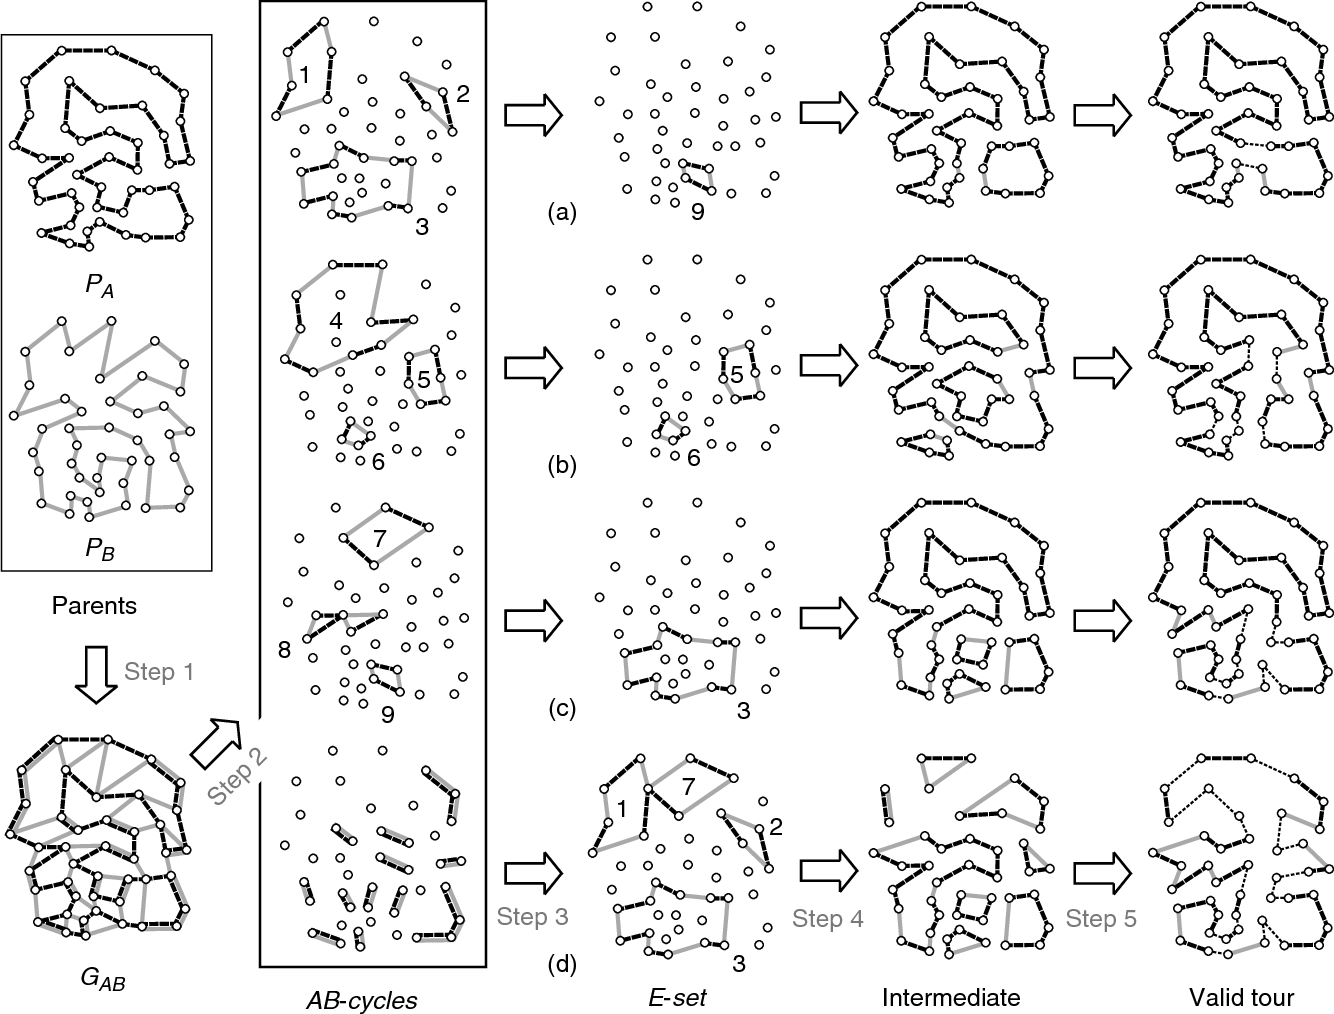
\includegraphics[width=1.0\columnwidth]{img/GA_steps}
	\caption{Example of the EAX\_SINGLE method steps (image taken from \cite{Nagata2013}).}
	\label{fig:GA_steps}
\end{figure}

Focusing on details of the EAX procedure:\\
Once two parents have been selected for crossover, the EAX operator merges these two individuals into a single graph denoted by R (Step 1 of Image \ref{fig:GA_steps}, graph R is named G\textsubscript{AB}). The two parents are denoted by A and B, respectively. Each edge in R is annotated with the parent to which it belongs. R may contain two instances of the same edge, if both parents contain the edge (that is why a more general version of Patching Algorithm is used).\\
R is next divided into a set of disjoint subtours. Let v\textsubscript{i} represent a vertex from R and let (v\textsubscript{i},  v\textsubscript{j}), i $\neq$ j, represent an edge. Suppose (v\textsubscript{i},  v\textsubscript{j}) represents an edge randomly chosen from parent A.\\
Choose one vertex (either v\textsubscript{i} or v\textsubscript{j}) as the origin. If v\textsubscript{i} is the origin, then choose an edge which leads from the second vertex, v\textsubscript{j} , to any other vertex in R. However, this edge must come from parent B. If more than one such edge exists, a random selection is made. The algorithm continues to traverse R, at each step alternately picking edges from parent A and parent B.\\
After each edge is traversed, the algorithm checks to see if adding this new edge to the set of previously selected edges will result in an AB-cycle. An AB-cycle is a even-length sub-cycle of R with edges that alternately come from A and B. An AB-cycle may repeat nodes, but not edges. While there can be two edges between a pair of nodes, they are uniquely identified as an A or B edge, and thus distinct.\\
Once an AB-cycle has been found it is stored and the edges making up that cycle are removed from R. The algorithm repeats this procedure until R contains no more edges, having been completely decomposed into a set of AB-cycles (Step 2 of Image \ref{fig:GA_steps}). \\
The first several edges used in the construction of the AB-cycle may not appear in the final AB-cycle. This occurs when the final edge connects back onto the subgraph at some node x other than the origin node, and the induced subcycle is an AB-cycle. In this case the remaining edges are however removed from R graph but is kept aside in the path being traced, to eventually be used later in forming another cycle. Nagata and Kobayashi choose an edge incident with x from R to begin construction of the next AB-cycle instead in our algorithm we preferred to take an edge incident to any node remaining in the traced path (other technique prefers to select the starting location of a new AB-cycle at random from R).
For the symmetric TSP problem, R is undirected and therefore, the set of AB-cycles is not uniquely determined by the algorithm. Furthermore, a number of "ineffective" AB-cycles may be formed by the algorithm. All AB-cycles that have less than 4 different nodes inside them belong to this group. Any ineffective AB-cycles are found and removed from R and also removed from consideration by the remaining phases of the algorithm.
\\
After construction of the set of AB-cycles, a subset of AB-cycles is chosen to be used in the generation of an intermediate child. This subset is called an E-set (Step 3 of Image \ref{fig:GA_steps}). For selecting AB-cycles for inclusion into the E-set, we choose an our method different from those defined by Nagata and Kobayashi. Given the small size of the problems we tested compared to those of the TSP Art of Nagata, the number of subtours in the E-set is not very large and therefore, instead of sampling by random selection some of them, we scroll through them all and create one intermediate child for each.
\\
Construction of an intermediate child, C, begins with a copy of parent A. Then each edge of each subtour in the E-set is examined, with the following actions taken on C. If the edge from the E-set is a member of parent A, the edge is deleted from C. If the edge is a member of parent B, the edge is added to C. The result is a set of disjoint subtours which comprise the intermediate child (Step 4 of Image \ref{fig:GA_steps}). \\
The last stage of the EAX operator involves transformation of the intermediate child into a single legal tour using a general Patching Algorithm (Step 5 of Image \ref{fig:GA_steps}). The difference between this general algorithm and the one presented in \ref{section:patching} is in the possibility of having double edges, after performing Step 4. This implies that one of the subtours can only be made up of two nodes and two same edges, one of parent A and one of B. Similar situation with three nodes and six edges (three doubles). In previous problems this situation never happened and therefore we generalized the Patching algorithm to include this variant.\\ 
The pseudocode of the EAX\_SINGLE method is identical to that explained in Algorithm 1 of Paper \cite{Honda2013}.

\subsection{Evaluate AB-Cycles}
This method was completely designed by us from scratch. It refers to how to find a cycle that respects the conditions of the EAX\_SINGLE procedure inside the nodes and edges traced so far by the current AB-Cycle. An explanation of this procedure is not given in the papers \cite{Nagata2013, Honda2013} and it is not even that simple. We initially thought of using a greedy graph search algorithm, such as Depth First Traversal (DFT) or Breadth First Search (BFS), but these algorithms do not include the presence of double edges between two nodes and are based on visiting the nodes and not edges and also once found any cycle they stop and do not provide the possibility to continue the search if the cycle does not meet certain conditions. So we have developed an ad hoc algorithm for this type of search that transforms the graph into a tree considering double edges and the possibility to continue the search if a cycle is found that does not respect the conditions required by the EAX\_SINGLE. This algorithm has a recursive structure and uses linked lists that allow a dynamic allocation to save all the necessary information, it was also built trying to free up memory as much as possible in order to avoid overflow as the generations increase. Furthermore, the possibility of finding all the cycles within the graph and not only one is managed, but, as required by the EAX, when an acceptable solution is found, the search ends.

\subsection{SURVIVAL\_SELECTION}
For the survival selection method, some parameters are defined: 

\begin{itemize}
\item N\textsubscript{pop}
\item N\textsubscript{kids}
\item Edge Frequency Table F($e$)
\end{itemize}
N\textsubscript{pop} and N\textsubscript{kids} be the population size and the number of offspring solutions generated from a single pair of parents, p\textsubscript{A} and p\textsubscript{B}, respectively, with the chosen values of 300 and 30, as in the default configuration of GA-EAX/Stage I \cite{Nagata2013}. N\textsubscript{kids} represents an upper bound to the number of offspring solutions but fewer of them could be generated. \\
The edge frequency table F($e$) is a table that records the frequencies of each edge $e \in E$ included in the population, where $E$ is the edge set of the complete graph of a given TSP instance. The values of F($e$) are initialized and are used in the evaluation function for selecting offspring solutions. This evaluation function is based on the edge entropy measure computed from F($e$) and is used for maintaining the population diversity in a positive manner. \\
To keep the table updated: let $y\ssymbol{1}$ be the selected individual among the generated offsprings, which replaces the population member chosen as parent p\textsubscript{A}. The values of F($e$) are updated as follows: 

\begin{equation}\begin{array}{ll}
F(e) \leftarrow F(e)-1 & \forall e \in E\textsubscript{remove} \\
F(e) \leftarrow F(e)+1 & \forall e \in E\textsubscript{add}
\end{array}\end{equation}

where E\textsubscript{remove} is a set of the edges that are included in p\textsubscript{A} but not included in $y\ssymbol{1}$, E\textsubscript{add} is a set of the edges that are included in $y\ssymbol{1}$ but not included in p\textsubscript{A}. \\

The offspring $y\ssymbol{1}$ is selected, taking account of the balance between the amount of the improvement and loss of the population diversity. Let L be the average tour length of the population and H the edge entropy of the population defined as follows:

\begin{equation}
H=-\sum_{e \in E} F(e) / N_{\mathrm{pop}}\left(\log \left(F(e) / N_{\mathrm{pop}}\right)\right)
\end{equation}

$\Delta$L(y) and $\Delta$H(y) denote the differences in L and H, respectively, when x\textsubscript{i}(p\textsubscript{A}) is replaced with $y\ssymbol{1}$. The offspring $y\ssymbol{1}$ is selected so that the following evaluation function is maximized.

\begin{equation}\text { Eval\textsubscript{Ent}}(y):=\left\{\begin{array}{ll}
\frac{\Delta L(y)}{\Delta H(y)} & (\Delta L<0, \Delta H<0) \\
-\frac{\Delta L(y)}{\epsilon} & (\Delta L<0, \Delta H \geq 0) \\
-\Delta L(y), & (\Delta L \geq 0)
\end{array}\right.\end{equation}

where $y$ is an offspring solution and $\epsilon$ is a sufficiently small positive number (our chosen value $0.1$).\\

\subsection{Test}

